
% a new beamer file for prague workshop

%% 
%%	This is file 'beamer_sample.tex'
%%	according to an MPIDR's PowerPoint template (?)
%%	
%%	by Eric Naujoks
%%
%%	Problems, bugs and comments to 
%%	naujoks@demogr.mpg.de
%%

%%%%%%%%%%%%%%%%%%%%%%%%%%%%%%%%%%
%%	Praelegomena								%%
%%%%%%%%%%%%%%%%%%%%%%%%%%%%%%%%%%
%%	- Make sure that you use utf8-encoding for all your .tex-files!!! (TeXnicCenter since version 2.0)
%%	- TeXnicCenter update: MPIDR intranet > Hard- & Sortfware > Software > Script and text editors > TeXnicCenter

\documentclass[20pt]{beamer}

\usepackage[ngerman,english]{babel}
\usepackage{graphicx}
\usepackage{tikz}
\usepackage{animate} 
\usepackage[normalem]{ulem}
\geometry{paperwidth=10in, paperheight=7.5in}
\usepackage{hyperref}
\usepackage[utf8]{inputenc}
\usepackage{movie15}
%\usepackage{multimedia}
\usepackage[mpidr]{./mpidr/beamerthemeMPIDR}


%% Declaring title and author
\title{Demographic time}
\subtitle{Tim Riffe\\ Jonas Sch{\"o}ley\\
Francisco Villavicencio}
%% subtitle means author in this file...
% :/
%%	the institute's logo
\renewcommand{\mylogo}{
\includegraphics[width=4.7in]{mpidr_logo_colour_en}}


%%	should be the very last package to be loaded
\usepackage{hyperref}

%%%%%%%%%%%%%%%%%%%%%%%%%%%%%%%%%%
%%	Beginning of the document		%%
%%%%%%%%%%%%%%%%%%%%%%%%%%%%%%%%%%
\begin{document}
%%	titlepage - fixed frame:
%%	========================
\begin{frame}
	\titlepage
\end{frame}

\begin{frame}%{Table of Contents}
\frametitle{Six time measures}
  \begin{description}
    \item<1->{\textbf{A}:} chronological age, time since birth
    \item<2->{\textbf{P}:} period, calendar year
    \item<3->{\textbf{C}:} birth cohort, calendar time of birth
    \item<4->{\textbf{T}:} thanatological age, time to death
    \item<5->{\textbf{D}:} death cohort, calendar time of death
    \item<6->{\textbf{L}:} lifespan, duration of life
    \end{description}
\end{frame}

% typical APC setup
\begin{frame}
\frametitle{A graph of time measures}
\begin{figure}[b]
    \centering
       % figure made in R/TetraCombos.R
    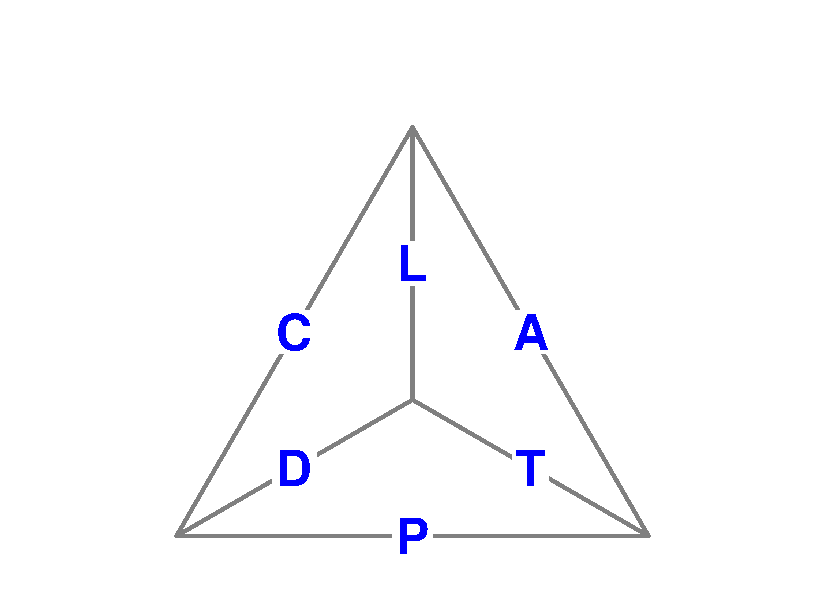
\includegraphics{Figures/Tetra1prg.pdf}
\end{figure} 
\end{frame}

%%	====
\begin{frame}%{Table of Contents}
\frametitle{~}
  \begin{description}
    \item<1->{\textbf{APC}:} aligned to time of birth, no death.
    \item<2->{\textbf{TPD}:} aligned to death, no birth
    \item<3->{\textbf{TAL}:} shows variation over the lifespan, but not in
    calendar time.
    \item<4->{\textbf{LCD}:} lifespans positioned in calendar time, but without
    age.
    \item<5->{\textbf{APCTDL}:} everything in one redundant 3d relationship.
  \end{description}
\end{frame}


%%	section 1:
%%	APC
\section{APC}
% past, observed, future
\begin{frame}
\frametitle{APC}
\vspace{-6em}
\begin{figure}
\raggedleft
    % figure made in R/TetraCombos.R
    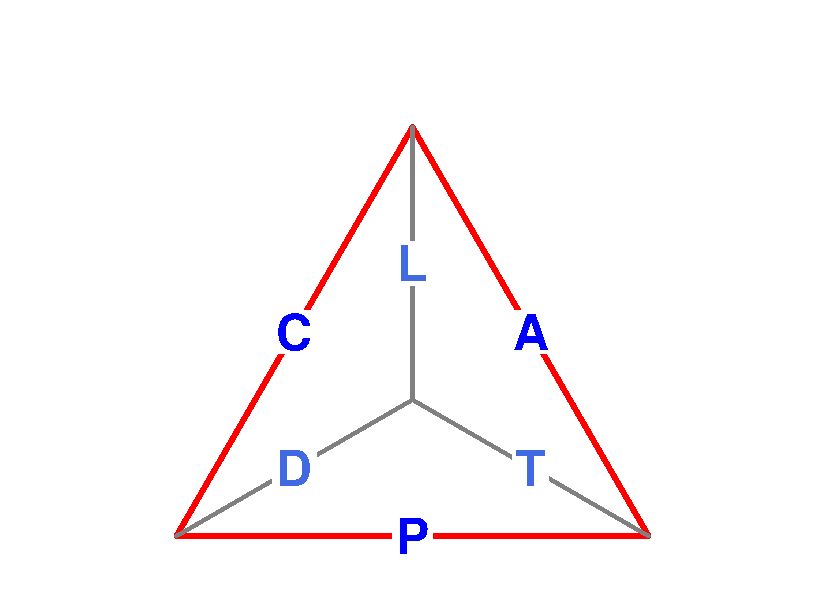
\includegraphics[scale=.7]{Figures/TetraAPCprg.pdf}
\end{figure}
\vspace{-3em}
\begin{figure}[b]
    \centering
       % figure made in R/APClab.R
    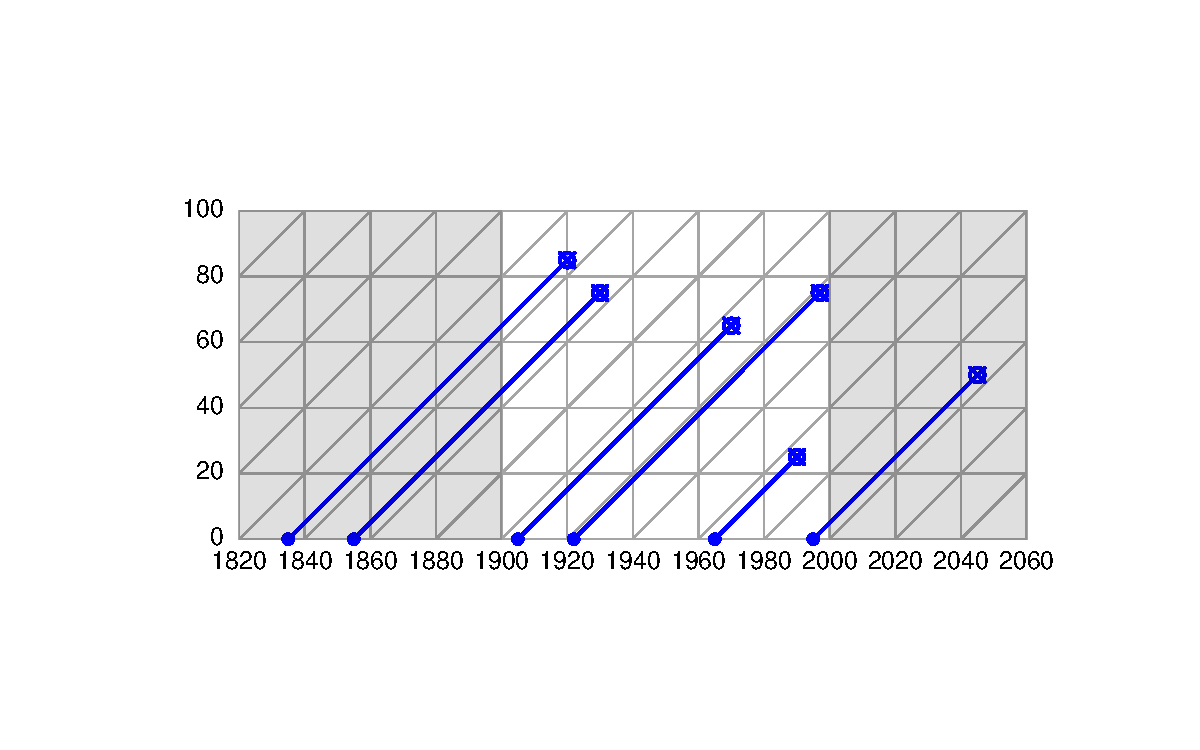
\includegraphics{Figures/LabPres/APC4.pdf}
   % \caption{Lifelines in the APC diagram, past and future}
\end{figure} 
\end{frame}

%%	TPD
\section{TPD}
\begin{frame} 
\frametitle{realign lifelines}
\begin{figure}
    \centering
  \animategraphics[height=5in]{36}{Figures/LabPres/AnimateLifeLines/frame_}{1}{95}
\end{figure} 
\end{frame} 

\begin{frame}
\frametitle{TPD, the inverse relationship}
\vspace{-6em}
\begin{figure}
\raggedleft
    % figure made in R/TetraCombos.R
    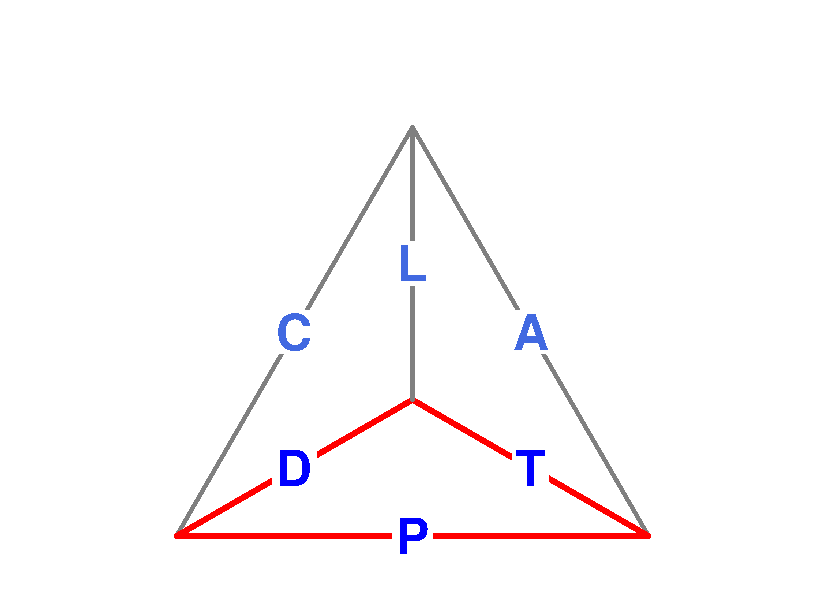
\includegraphics[scale=.7]{Figures/TetraTPDprg.pdf}
\end{figure}
\vspace{-3em}
\begin{figure}[b]
    \centering
    % figure made in R/TPDlab.R
    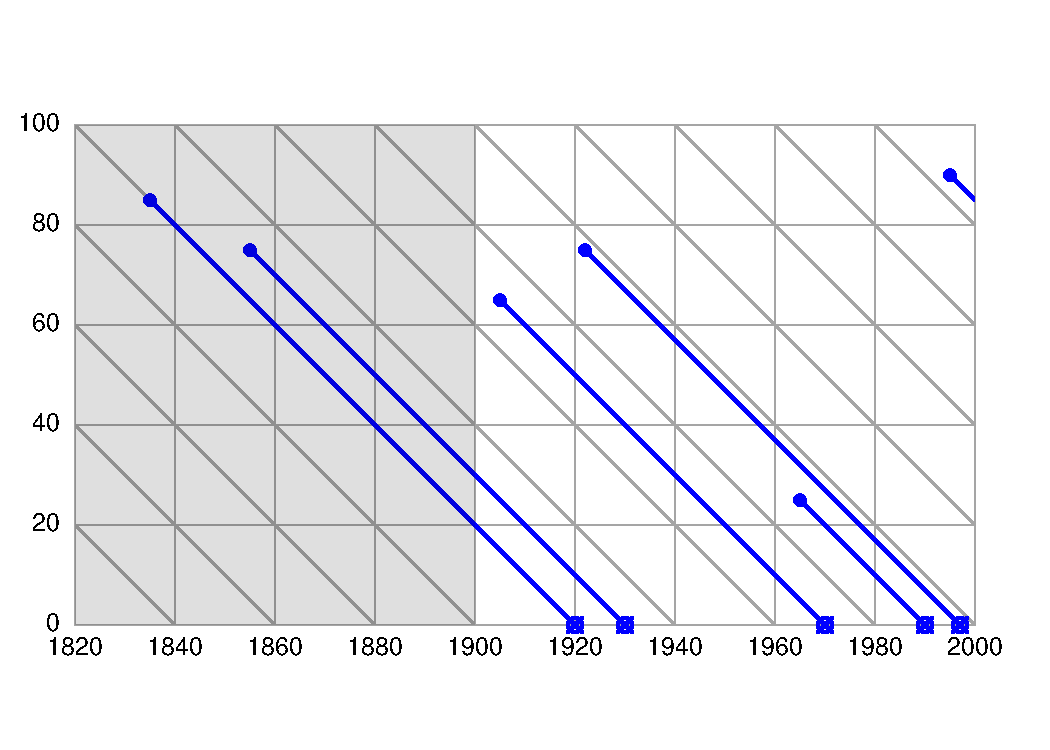
\includegraphics{Figures/LabPres/TPD2.pdf}
    %\caption{Lifelines in the TPD diagram}
\end{figure} 
\end{frame}

%%%%%%%%%%%%%%%%%%%%%%%%%%%%%%%%%%%%%%%%%%%%%%%
\section{TAL}
% with
\begin{frame}
\frametitle{TAL, a lifespan diagram}
\vspace{-5em}
\begin{figure}
\raggedleft
    % figure made in R/TetraCombos.R
    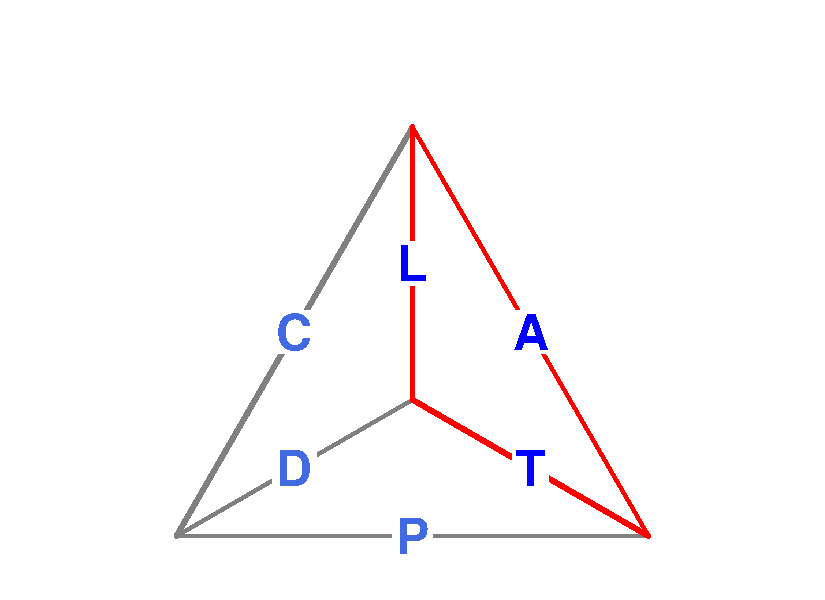
\includegraphics[scale=.7]{Figures/TetraTALprg.pdf}
\end{figure}
\vspace{-5em}
\begin{figure}[b]
    \centering
    % figure made in R/ATLlab.R
    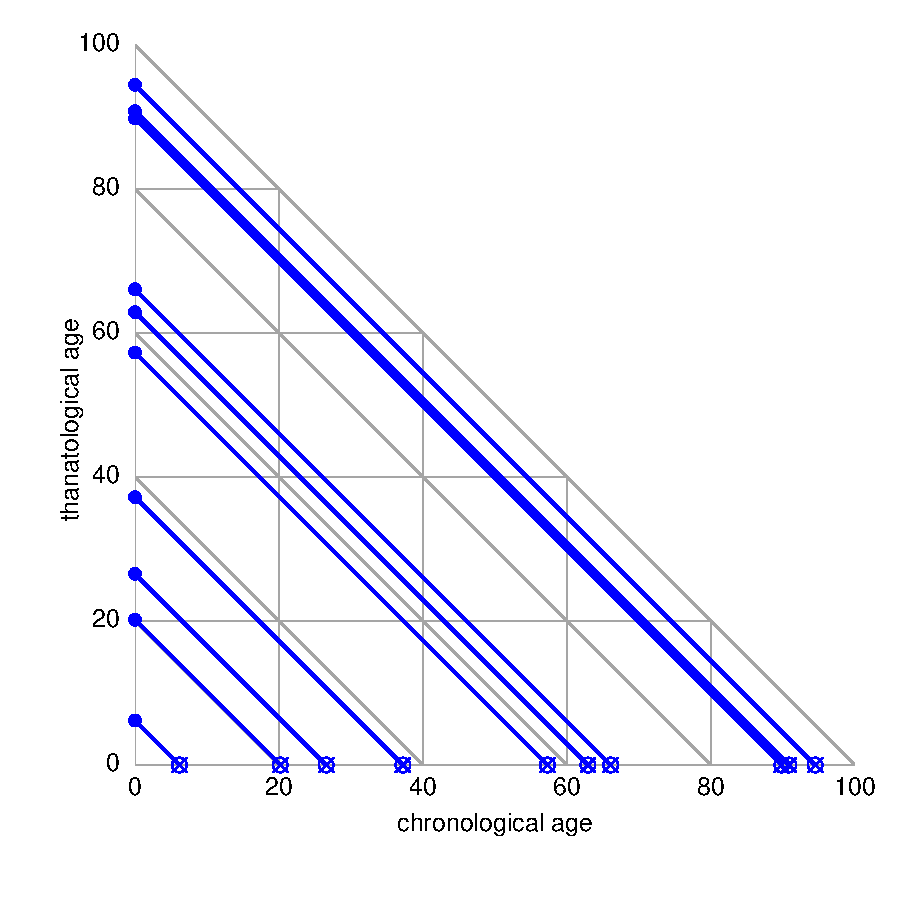
\includegraphics{Figures/LabPres/ATL2.pdf}
\end{figure} 
\end{frame}

\begin{frame}
\frametitle{TAL (cohort), spotted in the wild}
\begin{figure}[b]
    \centering
    % figure made in R/ATLlab.R
    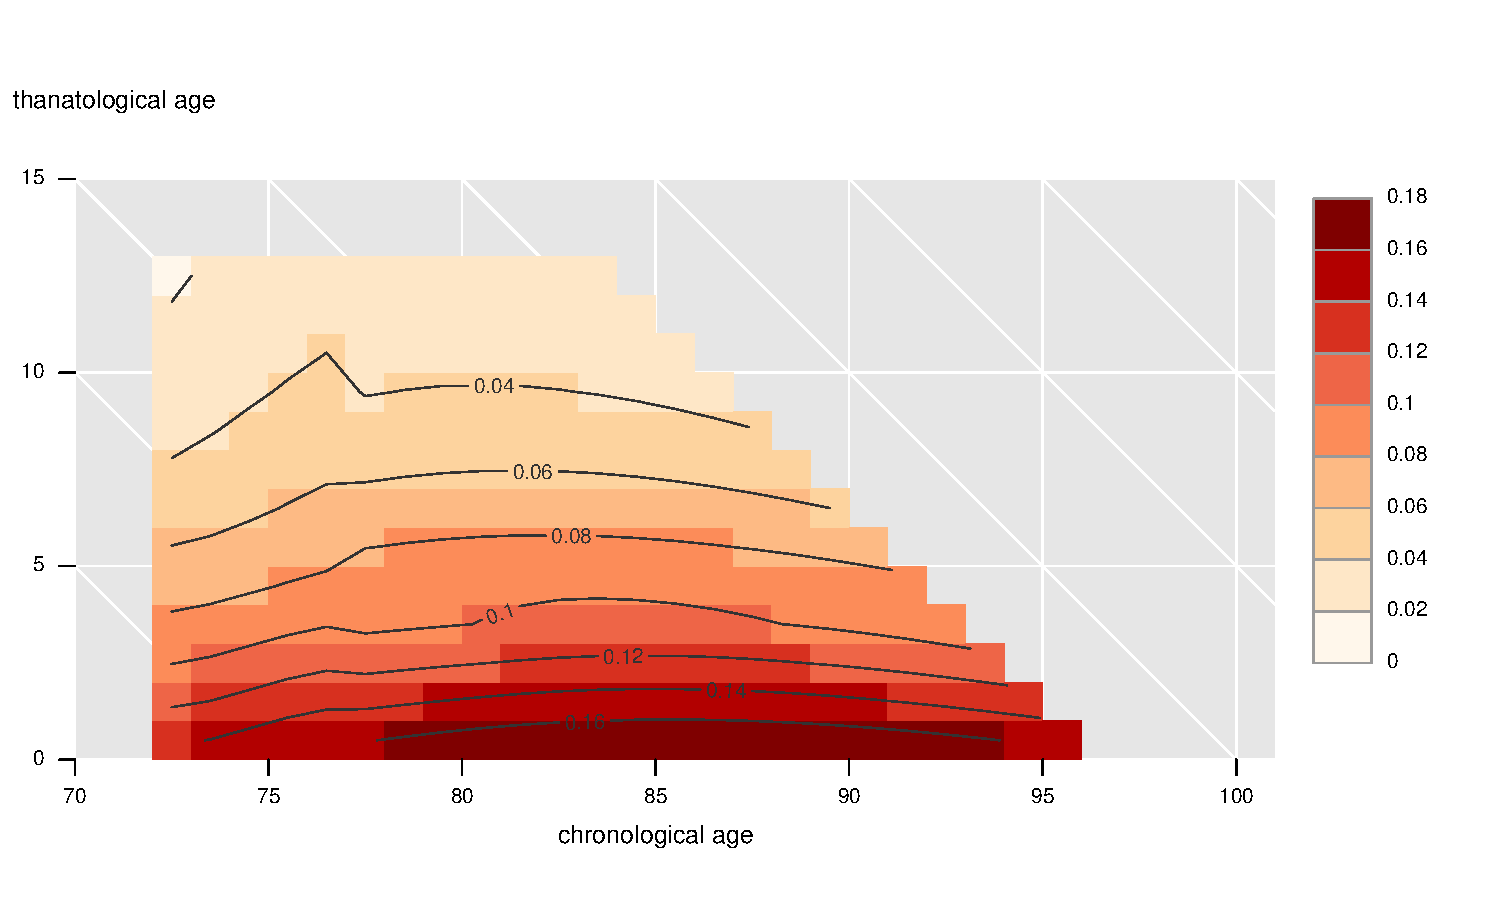
\includegraphics[scale=.9]{Figures/LabPres/ATL_Surf_Male_psych_HRS.pdf}
\end{figure} 
\end{frame}

\section{LCD}
\begin{frame}
\frametitle{LCD, a lifespan diagram}
\vspace{-6em}
\begin{figure}
\raggedleft
    % figure made in R/TetraCombos.R
    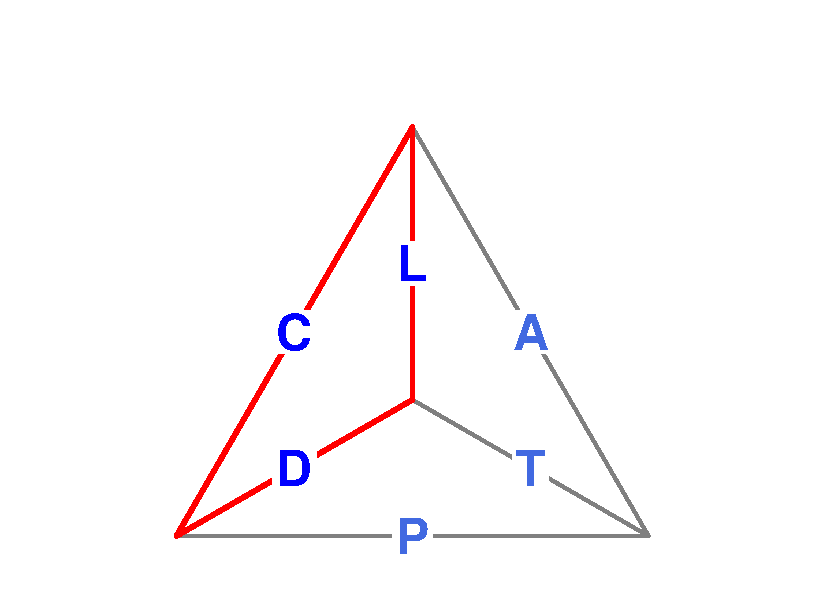
\includegraphics[scale=.7]{Figures/TetraLCDprg.pdf}
\end{figure}
\vspace{-3em}
\begin{figure}[b]
    \centering
    % figure made in R/ATLlab.R
    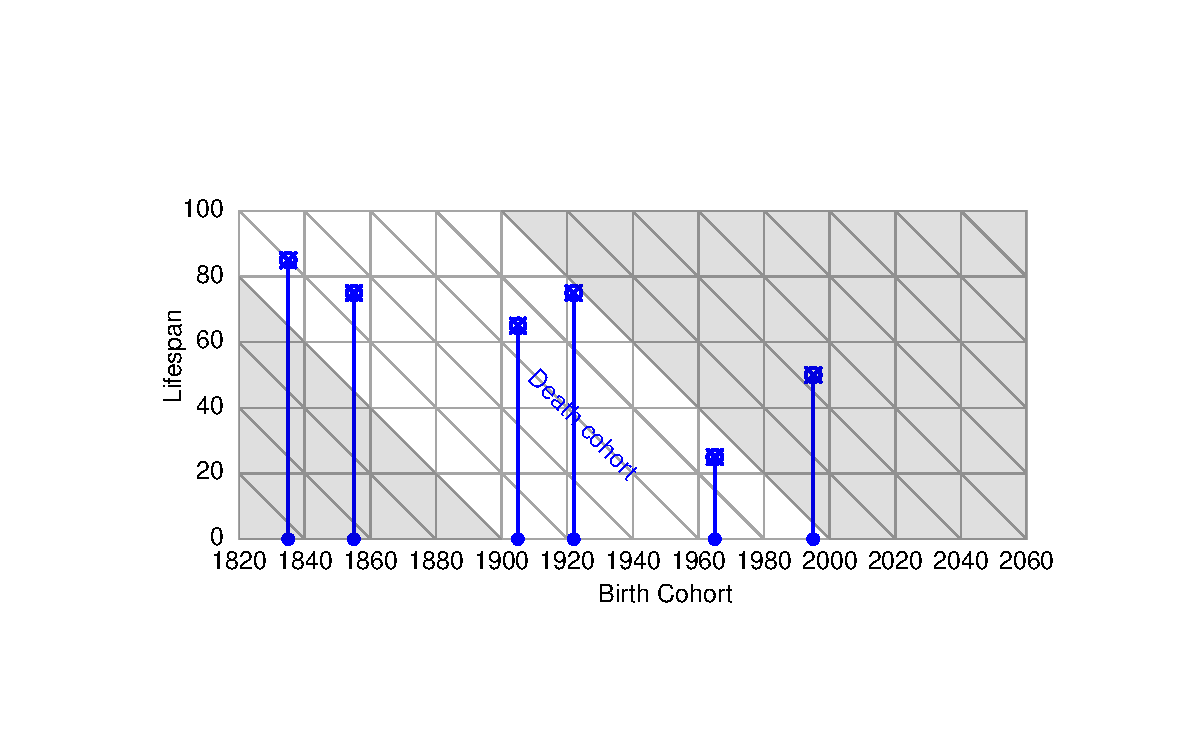
\includegraphics{Figures/LCD.pdf}
\end{figure} 
\end{frame}

\section{APCTDL}

\begin{frame}
\frametitle{A tetrahedron joins the diagrams}
\begin{figure}[b]
    \centering
       % figure made in R/TetraCombos.R
    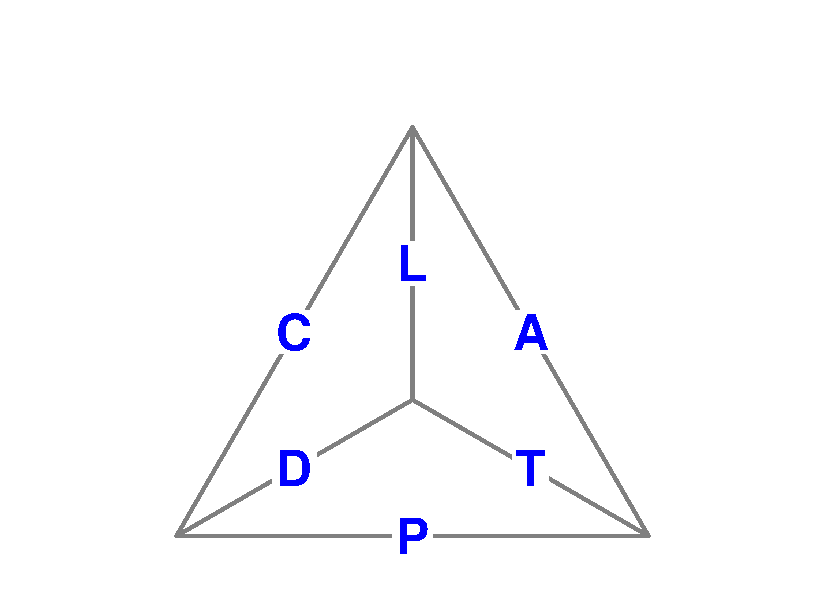
\includegraphics{Figures/Tetra1prg.pdf}
    \end{figure}
\end{frame}

\begin{frame}
\frametitle{All diagrams combined:}
Using right-angles (interactive, web):
\url{http://demog.berkeley.edu/~triffe/RGL1/}

\end{frame}

\begin{frame}
\frametitle{All diagrams combined:}

* As a regular honeycomb *

\end{frame}

\end{document}











